\section{Controlling a Physical Vehicle with \autofocus}
\label{sec:toy_rover_controller}

The model that we developed for the MDE tool challenge is based on a larger
model, that was originally created in the context of a lab course at Technical
University Munich. Two subsequent courses involving 10 students not only built
the logical model for the vehicle, but also the hardware platform of a car in
the scale of 1:10.
An important requirement for this vehicle was a high level of realism. Accordingly,
a professional platform with a realistic Ackermann steering and electrical all
wheel drive was chosen and configured in such a way that the driving
dynamics correspond to a realistic car. A picture of the vehicle is shown in
\fig\ref{fig:vehicle}.

\begin{figure}[!h]
\centering
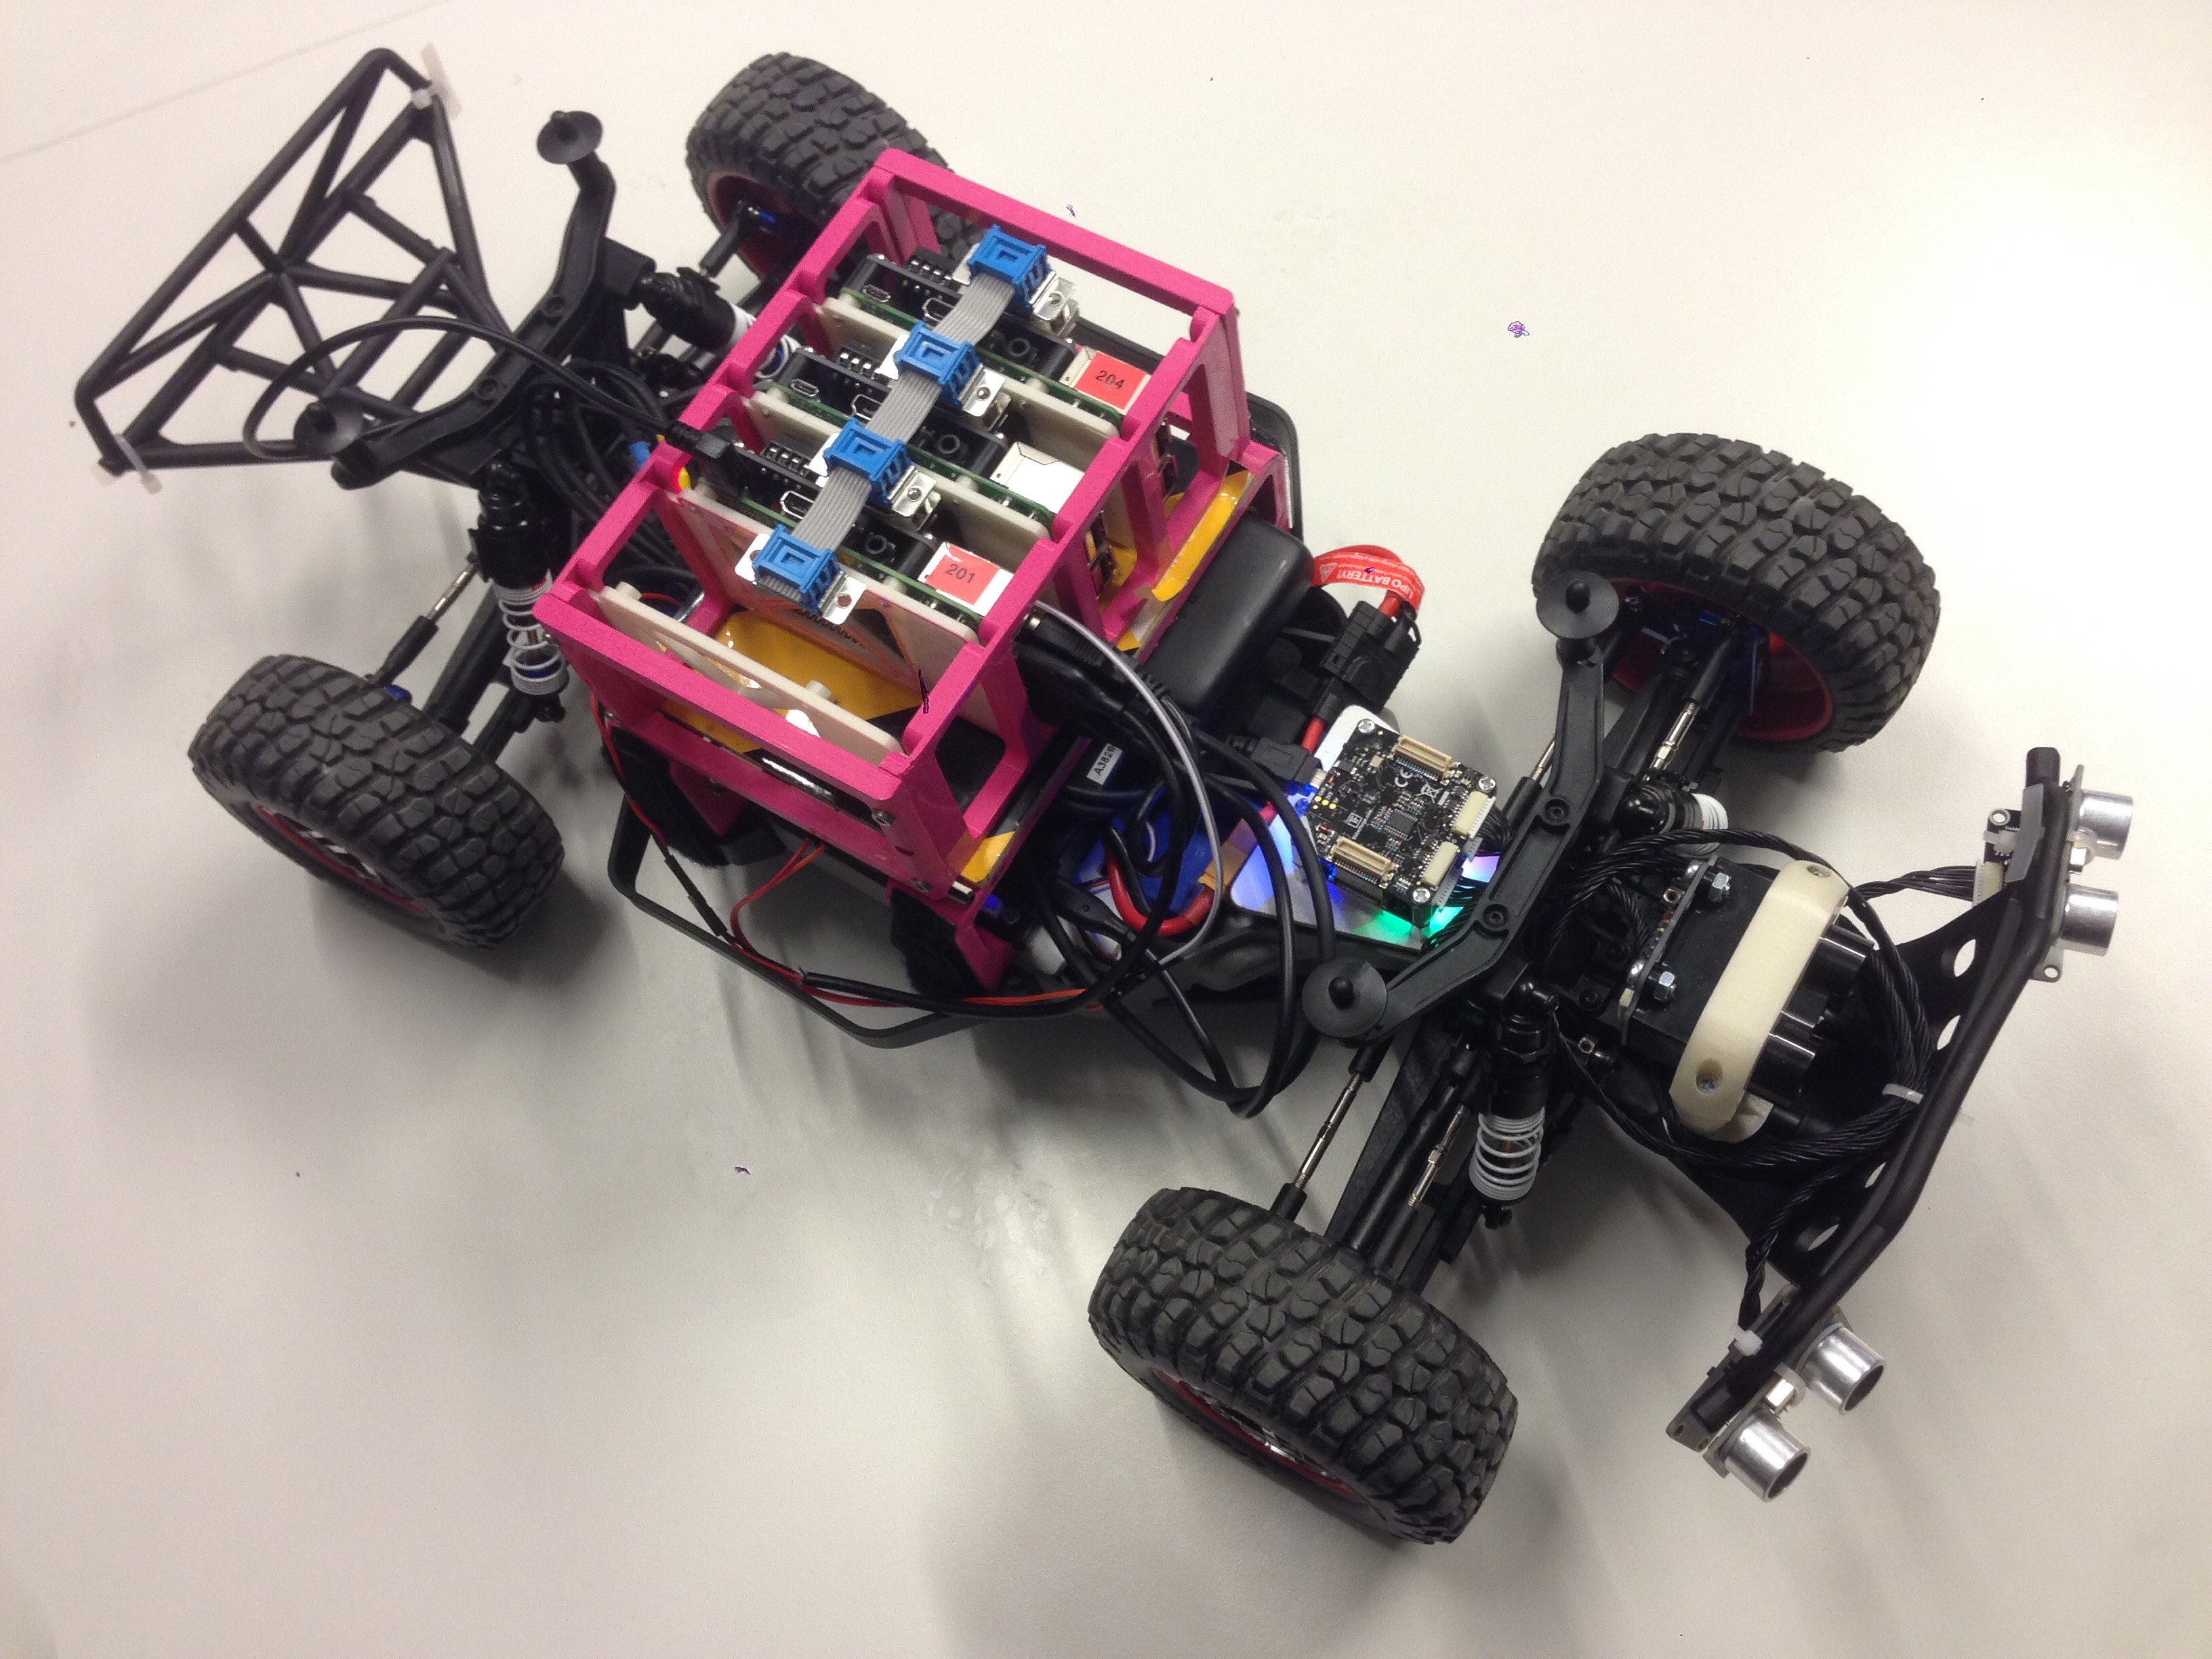
\includegraphics[width=1\textwidth]{images/FullSizeRender.jpg}
\caption{A Physical Rover used for a lab course at the Technical University
of Munich}
\label{fig:vehicle}
\end{figure}

The model that the students developed in the first lab course implemented basic
driving functionalities such as steering, braking, accelerating, gear shifting
and different drive modes, as well as two driver assistance functions for
emergency braking and adaptive cruise control.
The second lab course extended this outcome with lane keeping as well as
vehicle2vehicle communication and platooning.
Our main interest in the development of such a vehicle was to show the
applicability of model-based development by using our tool \autofocus on the one
hand, and on the other hand to come up with a software architecture for future
(semi-) autonomous cars. The general question we addressed was
how (semi-) autonomous functionality can be integrated into a software
architecture of a car, using a model-based approach. The current state of the
architecture is shown in \fig\ref{fig:vehicle_architecture} and is given as a
means to illustrate the complexity of the model of the controller developed by
the students.

\begin{figure}[!h]
\centering
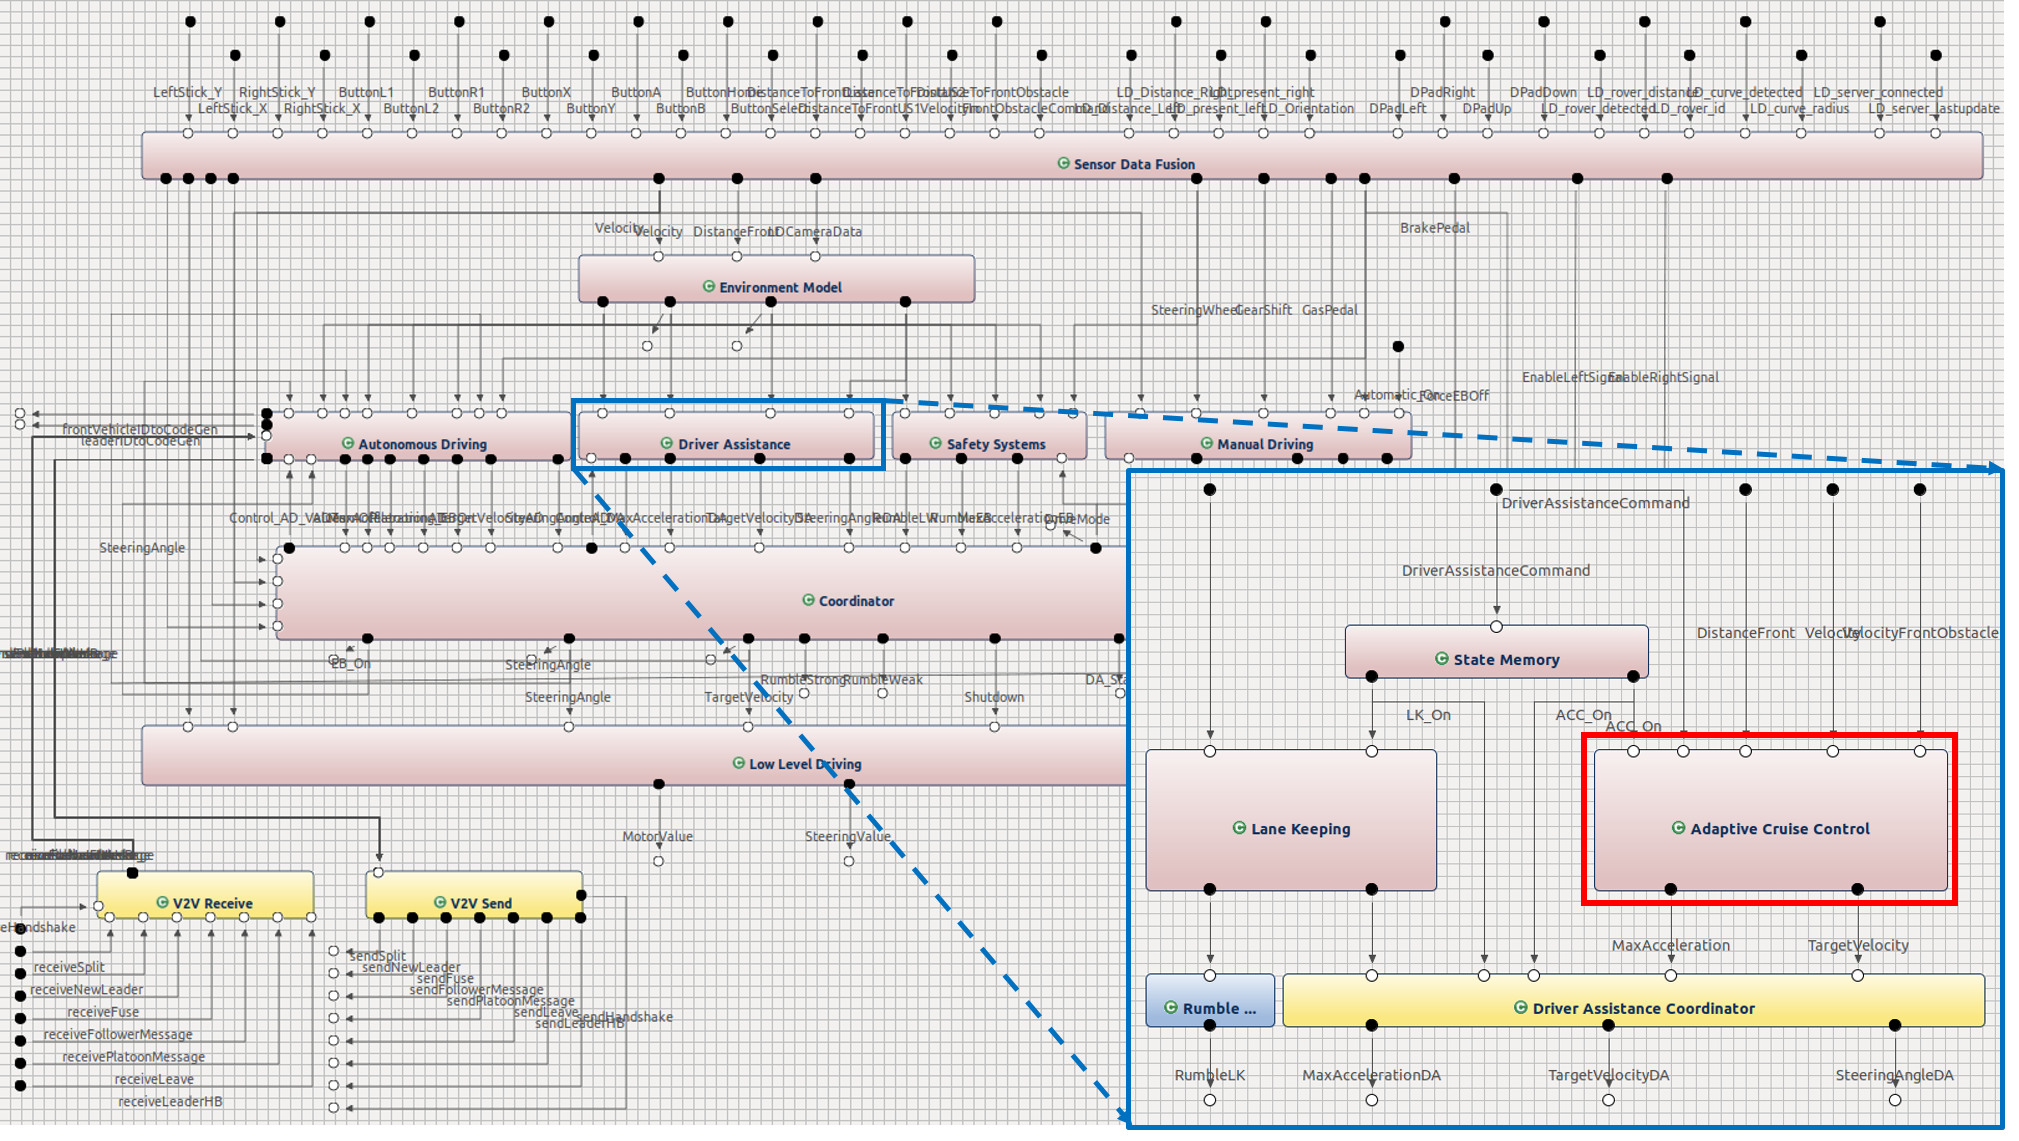
\includegraphics[width=1.4\textwidth, angle=90]{images/ACC_architecture}
\caption{The \af Model developed by the Students to Control a Physical Vehicle}
\label{fig:vehicle_architecture}
\end{figure}

For the MDE tool challenge we used the Adaptive Cruise Control (\acc) part of
the model, highlighted in  \fig\ref{fig:vehicle_architecture}. Because of the
component based approach of \af, we were able to reuse the component which
realized this function and adapt it to the challenge by developing against the
component's interface. Although we kept that part of the functionality that
adapts the distance to the leader rover, we had to incorporate in the model new
capabilities to allow automatic steering in order to implement the ``follow the
leader'' requirement. Naturally, we also had to adapt the inputs and the outputs of the
component to the data provided and expected by the virtual environment.
